%File: anonymous-submission-latex-2023.tex
\documentclass[letterpaper]{article} % DO NOT CHANGE THIS
\usepackage[submission]{aaai23}  % DO NOT CHANGE THIS
\usepackage{times}  % DO NOT CHANGE THIS
\usepackage{helvet}  % DO NOT CHANGE THIS
\usepackage{courier}  % DO NOT CHANGE THIS
\usepackage[hyphens]{url}  % DO NOT CHANGE THIS
\usepackage{graphicx} % DO NOT CHANGE THIS
\urlstyle{rm} % DO NOT CHANGE THIS
\def\UrlFont{\rm}  % DO NOT CHANGE THIS
\usepackage{natbib}  % DO NOT CHANGE THIS AND DO NOT ADD ANY OPTIONS TO IT
\usepackage{caption} % DO NOT CHANGE THIS AND DO NOT ADD ANY OPTIONS TO IT
\frenchspacing  % DO NOT CHANGE THIS
\setlength{\pdfpagewidth}{8.5in} % DO NOT CHANGE THIS
\setlength{\pdfpageheight}{11in} % DO NOT CHANGE THIS

\usepackage{mathtools}
\usepackage{amsthm}
\usepackage{mathrsfs}
\usepackage{amsfonts}
\usepackage{amssymb}
\usepackage{pifont}
\usepackage[linesnumbered,ruled,vlined]{algorithm2e}
\usepackage{tikz}
\usepackage[capitalize]{cleveref}
\usepackage{booktabs}
\usepackage{multirow}
\usepackage{colortbl}
\usepackage{subcaption}
\usepackage[inline,shortlabels]{enumitem}
\usepackage{complexity}

% These are recommended to typeset algorithms but not required. See the subsubsection on algorithms. Remove them if you don't have algorithms in your paper.
% \usepackage{algorithm}
% \usepackage{algorithmic}

% These are recommended to typeset listings but not required. See the subsubsection on listing. Remove this block if you don't have listings in your paper.
% \usepackage{newfloat}
% \usepackage{listings}
% \DeclareCaptionStyle{ruled}{labelfont=normalfont,labelsep=colon,strut=off} % DO NOT CHANGE THIS
% \lstset{%
% 	basicstyle={\footnotesize\ttfamily},% footnotesize acceptable for monospace
% 	numbers=left,numberstyle=\footnotesize,xleftmargin=2em,% show line numbers, remove this entire line if you don't want the numbers.
% 	aboveskip=0pt,belowskip=0pt,%
% 	showstringspaces=false,tabsize=2,breaklines=true}
% \floatstyle{ruled}
% \newfloat{listing}{tb}{lst}{}
% \floatname{listing}{Listing}

% Keep the \pdfinfo as shown here. There's no need
% for you to add the /Title and /Author tags.
\pdfinfo{
/TemplateVersion (2023.1)
}

% DISALLOWED PACKAGES
% \usepackage{authblk} -- This package is specifically forbidden
% \usepackage{balance} -- This package is specifically forbidden
% \usepackage{color (if used in text)
% \usepackage{CJK} -- This package is specifically forbidden
% \usepackage{float} -- This package is specifically forbidden
% \usepackage{flushend} -- This package is specifically forbidden
% \usepackage{fontenc} -- This package is specifically forbidden
% \usepackage{fullpage} -- This package is specifically forbidden
% \usepackage{geometry} -- This package is specifically forbidden
% \usepackage{grffile} -- This package is specifically forbidden
% \usepackage{hyperref} -- This package is specifically forbidden
% \usepackage{navigator} -- This package is specifically forbidden
% (or any other package that embeds links such as navigator or hyperref)
% \indentfirst} -- This package is specifically forbidden
% \layout} -- This package is specifically forbidden
% \multicol} -- This package is specifically forbidden
% \nameref} -- This package is specifically forbidden
% \usepackage{savetrees} -- This package is specifically forbidden
% \usepackage{setspace} -- This package is specifically forbidden
% \usepackage{stfloats} -- This package is specifically forbidden
% \usepackage{tabu} -- This package is specifically forbidden
% \usepackage{titlesec} -- This package is specifically forbidden
% \usepackage{tocbibind} -- This package is specifically forbidden
% \usepackage{ulem} -- This package is specifically forbidden
% \usepackage{wrapfig} -- This package is specifically forbidden
% DISALLOWED COMMANDS
% \nocopyright -- Your paper will not be published if you use this command
% \addtolength -- This command may not be used
% \balance -- This command may not be used
% \baselinestretch -- Your paper will not be published if you use this command
% \clearpage -- No page breaks of any kind may be used for the final version of your paper
% \columnsep -- This command may not be used
% \newpage -- No page breaks of any kind may be used for the final version of your paper
% \pagebreak -- No page breaks of any kind may be used for the final version of your paperr
% \pagestyle -- This command may not be used
% \tiny -- This is not an acceptable font size.
% \vspace{- -- No negative value may be used in proximity of a caption, figure, table, section, subsection, subsubsection, or reference
% \vskip{- -- No negative value may be used to alter spacing above or below a caption, figure, table, section, subsection, subsubsection, or reference

\setcounter{secnumdepth}{2} %May be changed to 1 or 2 if section numbers are desired.

% Title

% Your title must be in mixed case, not sentence case.
% That means all verbs (including short verbs like be, is, using,and go),
% nouns, adverbs, adjectives should be capitalized, including both words in hyphenated terms, while
% articles, conjunctions, and prepositions are lower case unless they
% directly follow a colon or long dash
\title{Recursive Solutions to First-Order Model Counting}
\author{Anonymous Submission}
\affiliations{}

\captionsetup[subfigure]{width=\linewidth}
\usetikzlibrary{fit,positioning,trees,cd}
\usetikzlibrary{shapes}
\usetikzlibrary{arrows}
\usetikzlibrary{arrows.meta}
\newcommand{\crefrangeconjunction}{--}
\crefname{algocf}{algorithm}{Algorithms}
\Crefname{algocf}{Algorithm}{Algorithms}
\newcommand\pfun{\mathrel{\ooalign{\hfil$\mapstochar\mkern5mu$\hfil\cr$\to$\cr}}}
\newcommand\mdoubleplus{\mathbin{+\mkern-10mu+}}
\newcommand*{\twoheadrightarrowtail}{\mathrel{\rightarrowtail\kern-1.9ex\twoheadrightarrow}}
\newcommand{\cmark}{\ding{51}}%
\newcommand{\xmark}{\ding{55}}%
\newcommand{\FOtwo}{$\mathsf{FO}^{2}$}
\newcommand{\FOthree}{$\mathsf{FO}^{3}$}
\newcommand{\SFO}{$\mathsf{S}^{2}\mathsf{FO}^{2}$}
\newcommand{\SRU}{$\mathsf{S}^{2}\mathsf{RU}$}
\newcommand{\Uone}{$\mathsf{U}_{1}$}
\newcommand{\Ctwo}{$\mathsf{C}^{2}$}
\DeclareMathOperator{\CR}{\textsc{CR}}
\DeclareMathOperator{\GDR}{\textsc{GDR}}
\DeclareMathOperator{\IE}{\textsc{IE}}
\DeclareMathOperator{\Reff}{\textsc{Ref}}
\DeclareMathOperator{\wwp}{w}
\DeclareMathOperator{\wwn}{\overline{w}}
\DeclareMathOperator{\dom}{dom}
\DeclareMathOperator{\id}{id}
\DeclareMathOperator{\Imm}{Im}
\DeclareMathOperator{\Doms}{Doms}
\DeclareMathOperator{\size}{\sigma}
\DeclareMathOperator{\Vars}{Vars}
\DeclareMathOperator{\WMC}{WMC}
\DeclareMathOperator{\gr}{gr}
\DeclareMathOperator{\leftlsquigarrow}{\text{\reflectbox{$\rightsquigarrow$}}}
\SetKw{KwRet}{yield}
\SetKwProg{Fn}{Function}{:}{}
\SetKwFunction{applyAllRules}{applyAllRules}
\SetKwFunction{applyGreedyRules}{applyGreedyRules}
\SetKwFunction{applyGreedyRulesToFormulas}{applyGreedyRulesToFormulas}
\SetKwFunction{emptyy}{empty}
\SetKwFunction{get}{get}
\SetKwFunction{put}{put}
\SetKwFunction{constructDomainMap}{constructDomainMap}
\SetKwFunction{identifyRecursion}{identifyRecursion}
\SetKwFunction{generateMaps}{generateMaps}
\SetKwFunction{mergeFcgs}{mergeFcgs}
\SetKwFunction{updateCache}{updCache}
\newtheorem{assumption}{Assumption}
\newtheorem{conjecture}{Conjecture}
\newtheorem{constraint}{Constraint}
\newtheorem{fact}{Fact}
\newtheorem{proposition}{Proposition}
\newtheorem{theorem}{Theorem}
\newtheorem{lemma}{Lemma}
\theoremstyle{definition}
\newtheorem{definition}{Definition}
\newtheorem{example}{Example}
\newtheorem{experiment}{Experiment}
\theoremstyle{remark}
\newtheorem*{remark}{Remark}
\makeatletter
\newcommand{\nosemic}{\renewcommand{\@endalgocfline}{\relax}}% Drop semi-colon ;
\newcommand{\dosemic}{\renewcommand{\@endalgocfline}{\algocf@endline}}% Reinstate semi-colon ;
\newcommand{\pushline}{\Indp}% Indent
\newcommand{\popline}{\Indm\dosemic}% Undent
\makeatother
\Crefname{algocf}{Algorithm}{Algorithms}
\Crefname{constraint}{Constraint}{Constraints}
\Crefname{experiment}{Experiment}{Experiments}
\Crefname{clause}{Clause}{Clauses}
\Crefname{diagram}{Diagram}{Diagrams}
\crefname{line}{line}{lines}

\begin{document}

\maketitle

\begin{abstract}
  First-order model counting (FOMC) is a computational problem that asks to
  count the models of a sentence in first-order logic. Despite being around for
  more than a decade, practical FOMC algorithms are still unable to compute
  functions as simple as a factorial. We argue that the capabilities of FOMC
  algorithms are severely limited by their inability to express arbitrary
  recursive computations. To enable arbitrary recursion, we relax the
  restrictions that typically accompany domain recursion and generalise circuits
  used to express a solution to an FOMC problem to graphs that may contain
  cycles. To this end, we enhance the most well-established (weighted) FOMC
  algorithm ForcLift with new compilation rules and an algorithm to check
  whether a recursive call is feasible. These improvements allow us to find
  efficient solutions to counting fundamental structures such as injections and
  bijections.
\end{abstract}

\section{Introduction}

% 1. What is the problem?
% 2. Why is it interesting and important?
% 1) the latest first-order variable elimination algorithm \citep{DBLP:journals/jair/TaghipourFDB13}
% 2) other approaches to lifted inference  \citep{DBLP:conf/uai/BrazO17,DBLP:conf/nips/JhaGMS10,DBLP:journals/ijar/RiguzziBZCL17}
% 3) Unlike most early algorithms for lifted inference that were adaptations of probabilistic inference algorithms such as AND/OR search \citep{DBLP:conf/aaai/GogateD10} and variable elimination \citep{DBLP:conf/ijcai/BrazAR05,DBLP:conf/aaai/MilchZKHK08}, WFOMC is an approach grounded in logic.

\emph{First-order model counting} (FOMC) is the problem of computing the number
of models of a sentence in first-order logic (FOL) given the size(s) of its
domain(s) \citep{DBLP:conf/pods/BeameBGS15}. \emph{Symmetric weighted FOMC}
(WFOMC) extends FOMC with (pairs of) weights on predicates and asks for a
weighted sum across all models instead. WFOMC emerged as the dominant approach
to \emph{lifted (probabilistic) inference}. Lifted inference techniques exploit
symmetries in probabilistic models by reasoning about sets rather than
individuals \citep{DBLP:conf/ecai/Kersting12}. By doing so, many instances
become solvable in polynomial time \citep{DBLP:conf/nips/Broeck11}. Lifted
inference algorithms are typically used on probabilistic models such as
probabilistic programming languages
\citep{DBLP:journals/ml/RaedtK15,DBLP:journals/ijar/RiguzziBZCL17}, Markov logic
networks
\citep{DBLP:conf/ijcai/BroeckTMDR11,DBLP:journals/cacm/GogateD16,DBLP:journals/ml/RichardsonD06},
and other lifted graphical \citep{DBLP:journals/ml/KimmigMG15} and statistical
relational \citep{DBLP:series/synthesis/2016Raedt} models. Lifted inference
techniques for probabilistic databases, while developed somewhat independently,
have also been inspired by WFOMC
\citep{DBLP:journals/pvldb/GatterbauerS15,DBLP:journals/debu/GribkoffSB14}.

% 3. Why is it hard? (E.g., why do naive approaches fail?)
% complexity/liftability -> murky boundary

Traditionally in computational complexity theory, a problem is \emph{tractable}
if it can be solved in time polynomial in the size of the instance. The
equivalent notion in (W)FOMC is liftability. A (W)FOMC instance is
\emph{(domain-)liftable} if it can be solved in time polynomial in the size(s)
of the domain(s) \citep{jaeger2012liftability}. Over more than a decade, more
and more classes of instances were shown to be liftable
\citep{DBLP:conf/kr/BremenK21,DBLP:conf/nips/KazemiKBP16,DBLP:conf/lics/KuusistoL18,DBLP:journals/jair/Kuzelka21}.
First, \citet{DBLP:conf/nips/Broeck11} showed that the class of all sentences of
FOL with up to two variables (denoted \FOtwo{}) is liftable. Then
\citet{DBLP:conf/pods/BeameBGS15} proved that there exists a sentence with three
variables for which FOMC is $\#\P_{1}$-complete (i.e., \FOthree{} is not
liftable). Since these two results came out, most of the research on (W)FOMC
focused on developing faster solutions for the \FOtwo{} fragment
\citep{DBLP:conf/uai/BremenK21,DBLP:conf/aaai/MalhotraS22} and defining
new liftable fragments. These fragments include \SFO{} and \SRU{}
\citep{DBLP:conf/nips/KazemiKBP16}, \Uone{} \citep{DBLP:conf/lics/KuusistoL18},
\FOtwo{} with tree axioms \citep{DBLP:conf/kr/BremenK21}, and \Ctwo{} (i.e., the
two variable fragment with counting quantifiers)
\citep{DBLP:journals/jair/Kuzelka21,DBLP:conf/aaai/MalhotraS22}. On the
empirical front, there are several open-source implementations of exact WFOMC
algorithms: \textsc{ForcLift} \citep{DBLP:conf/ijcai/BroeckTMDR11},
probabilistic theorem proving \citep{DBLP:journals/cacm/GogateD16}, and
\textsc{L2C} \citep{DBLP:conf/kr/KazemiP16}. Approximate counting is supported
by \textsc{ApproxWFOMC} \citep{DBLP:conf/ijcai/BremenK20} as well as
\textsc{ForcLift} \citep{DBLP:conf/uai/BroeckCD12} and probabilistic theorem
proving \citep{DBLP:journals/cacm/GogateD16}.

% 4. Why hasn't it been solved before? (Or, what's wrong with previous proposed
% solutions? How does mine differ?)
% simple unliftable instances -> recursion

However, none of the publicly available exact (W)FOMC algorithms can efficiently
compute functions as simple as a factorial.\footnote{The problem of computing
  the factorial can be described using two variables and counting quantifiers,
  so it is known to be liftable in theory \citep{DBLP:journals/jair/Kuzelka21}.}
We claim that this shortcoming is due to the inability of these algorithms to
construct recursive solutions. The topic of recursion in the context of WFOMC
has been studied before but in limited ways.
\Citet{DBLP:conf/ilp/BarvinekB0ZK21} use WFOMC to generate numerical data which
is then used to conjecture recurrence relations that explain that data.
\Citet{DBLP:conf/nips/Broeck11} introduced the idea of \emph{domain recursion}.
Intuitively, domain recursion partitions a domain of size $n$ into a single
explicitly named constant and the remaining domain of size $n-1$. However, many
stringent conditions are enforced to ensure that the search for a tractable
solution always terminates.

% \begin{itemize}
%   \item But their code only conjectures stuff on data. My conjectures are
%         guaranteed to always be true.
%   \item everything has to be expressible in \Ctwo{}, i.e., the two-variable
%         fragment of FOL with counting quantifiers on one domain.
%   \item They only consider P-recursive functions, which means that, e.g.,
%         $f(n) = f(n-1)f(n-2)$ would not be allowed.
% \end{itemize}

% 5. What are the key components of my approach and results? Also include any
% specific limitations.

% 5.1) An overview of how ForcLift/Crane work.

In this work, we show how to relax these restrictions in a way that results in a
stronger (W)FOMC algorithm, capable of handling more instances in a lifted
manner. The ideas presented in this paper are implemented in
\textsc{Crane}---an extension of the arguably most well-known WFOMC algorithm
\textsc{ForcLift} written in Scala. \textsc{ForcLift} works in two stages:
compilation and evaluation/propagation.\footnote{There is also an intermediate
  stage called \emph{smoothing} that takes place between compilation and
  evaluation. As our changes to smoothing are quite elementary, we do not
  discuss them to not distract the reader from the main contributions of this
  paper.} In the first part, various \emph{(compilation) rules} are applied to
the input (or some derivative) formula, gradually constructing a circuit. In the
second part, the weights of the instance (and sometimes constants) are
propagated through the circuit, computing the WMC\@.

% 5.2) The main idea: cycles that represent recursive calls.

TODO: improve the wording of the paragraph below.

The main conceptual difference between \textsc{Crane} and \textsc{ForcLift} is
that we utilise labelled directed graphs instead of circuits. The cycles in
these graphs represent recursive calls. Suppose the original formula $\phi$
depends on a domain of size $n \in \mathbb{N}$. Our generalised version of
domain recursion transforms $\phi$ into a different formula $\psi$ that depends
on a domain of size $n-1$. After some number of subsequent transformations, the
algorithm identifies that a solution to $\psi$ can be constructed in part by
finding a solution to a version of $\phi$ where the domain of size $n$ is
replaced by a domain of size $n-1$. Recognising $\phi$ from before, we can add a
cycle-forming edge to the graph, which can be interpreted as function $f$
relying on $f(n-1)$ to compute $f(n)$.

% 5.3) contributions, references to sections, shortcomings

To construct such graphs, we introduce a novel search algorithm that replaces
greedy search used by \textsc{ForcLift} and three compilation rules that work
together to construct cyclic graphs. We begin with \cref{sec:recprelims} where
we define the representation used for sentences in FOL as well as discuss
caching and some notational conventions. Then, at the beginning of
\cref{sec:methods} we formally define the graphs that replace circuits in
representing a solution to a (W)FOMC problem and discuss some related notions.
\Cref{sec:rules} introduces the new compilation rules:
\begin{itemize}
  \item a generalisation of domain recursion by \citet{DBLP:conf/nips/Broeck11},
  \item \emph{constraint removal}---a formula transformation rule that removes
        the constraints introduced by generalised domain recursion (GDR),
        introducing a new (smaller) domain instead,
  \item and a rule for creating recursive calls.
\end{itemize}
In a typical solution produced by \textsc{Crane}, these rules are executed in
exactly this order (interspersed with some other rules), with the edge that
represents a recursive call pointing back to the node introduced by GDR\@. In
\cref{sec:interpret}, we informally discuss how a graph can be interpreted as a
collection of (potentially recursive) functions. Finally, in \cref{sec:results}
we compare \textsc{ForcLift} and \textsc{Crane} on a range of function-counting
problems. We show that \textsc{Crane} performs as well as \textsc{ForcLift} on
the instances that were already solvable by \textsc{ForcLift} but is also able
to handle most instances that \textsc{ForcLift} fails on as well.

% \Cref{sec:search} then describes our new search algorithm that makes fewer
% assumptions than \textsc{ForcLift} about the right order in which compilation
% rules should be applied.

% \begin{itemize}
%   \item What we do with the compilation result is different (see below)
%   \item evaluation/interpretation: algebraic simplification, dynamic programming
%   \item limitation: function extraction and simplification need to be automated,
%         same for finding base cases
% \end{itemize}

% Leftovers
% \begin{itemize}
%   \item compilation works by always having a formula as input and
%         adding nodes to the circuit/FCG that constitute the solution the that
%         formula.
%   \item Workflow after
%   \begin{itemize}
%     \item Compile the formula to a graph
%     \item Extract the definitions of functions
%     \item Simplify
%     \item Supplement with base cases
%     \item Evaluate to get the answer
%   \end{itemize}
% \end{itemize}

\section{Preliminaries}\label{sec:recprelims}

In this section, we describe our format for FOMC instances, introduce some
notation, and discuss our caching scheme, which is used to identify
possibilities for a recursive call. Note that although the focus of this paper
is on unweighted model counting, \textsc{ForcLift}'s
\citep{DBLP:conf/ijcai/BroeckTMDR11} support for weights trivially transfers to
\textsc{Crane} as well.

Our representation of FOMC instances is heavily based on the format used
internally by \textsc{ForcLift}, some aspects of which are described by
\citet{DBLP:conf/ijcai/BroeckTMDR11}. \textsc{ForcLift} is able to translate
sentences in a variant of function-free many-sorted FOL with equality to this
internal format. An \emph{atom} is $p(t_1, \dots, t_n)$ for some predicate $p$
and terms $t_{1}, \dots, t_{n}$. Here, $n \in \mathbb{N}_0$ is the \emph{arity}
of $p$. A \emph{term} is either a constant or a variable. A \emph{literal} is
either an atom or the negation of an atom (denoted by
$\neg p(t_1, \dots, t_n)$). Let $\mathcal{D}$ be the set of all domains; note
that this set expands during compilation.

\begin{definition}[Constraint]\label{def:constraint}
  An \emph{(inequality) constraint} is a pair $(a, b)$, where $a$ is a variable,
  and $b$ is either a variable or a constant.
\end{definition}

\begin{definition}[Clause]\label{def:clause}
  A \emph{clause}\footnote{\citet{DBLP:conf/ijcai/BroeckTMDR11} refer to clauses
    as c-clauses.} is a triple $c = (L, C, \delta_c)$, where $L$ is a set of
  literals, $C$ is a set of constraints, and $\delta_c$ is the domain map of
  $c$. Let $\Vars$ be the function that maps clauses and sets of either literals
  or constraints to the set of variables contained within. In particular,
  $\Vars(c) \coloneqq \Vars(L) \cup \Vars(C)$. \emph{Domain map}
  $\delta_{c}\colon \Vars(c) \to \mathcal{D}$ is a function that maps all
  variables in $c$ to their domains such that (s.t.) if $(X, Y) \in C$ for some
  variables $X$ and $Y$, then $\delta_c(X) = \delta_c(Y)$. For convenience, we
  sometimes write $\delta_c$ for the domain map of $c$ without unpacking $c$
  into its three constituents.
\end{definition}

Similarly to variables in \cref{def:clause}, all constants are (implicitly)
mapped to domains, and each $n$-ary predicate is implicitly mapped to a sequence
of $n$ domains. For constant $x$, predicate $p$, and domains $a$ and $b$, we
write, e.g., $x \in a$ and $p \in a \times b$ to denote that $x$ is associated
with $a$, and $p$ is associated with $a$ and $b$ (in that order).

\begin{definition}[Formula]\label{def:formula}
  A \emph{formula} (called a c-theory by \citet{DBLP:conf/ijcai/BroeckTMDR11})
  is a set of clauses such that all constraints and atoms `type check' with
  respect to domains.
\end{definition}

\begin{example}\label{example:first}
  Let $\phi \coloneqq \{\, c_1, c_2 \,\}$ be a formula with clauses
  \begin{align*}
    c_1 &\coloneqq
          \begin{multlined}[t]
            (\{\, \neg p(X, Y), \neg p(X, Z) \,\}, \{\, (Y, Z) \,\}, \\
            \{\, X \mapsto a, Y \mapsto b, Z \mapsto b \,\}),
          \end{multlined}\\
    c_2 &\coloneqq
          \begin{multlined}[t]
            (\{\, \neg p(X, Y), \neg p(Z, Y) \,\}, \{\, (X, Z) \,\}, \\
            \{\, X \mapsto a, Y \mapsto b, Z \mapsto a \,\})
          \end{multlined}
  \end{align*}
  for some predicate $p$, variables $X$, $Y$, $Z$, and domains $a$ and $b$. Then
  $\Vars(\{\, (Y, Z) \,\}) = \{\, Y, Z \,\}$, and
  $\Vars(c_{1}) = \Vars(c_{2}) = \{\, X, Y, Z \,\}$. Based on the domain maps of
  $c_{1}$ and $c_{2}$, we can infer that $p \in a \times b$. All variables (in
  both clauses) that occur as the first argument to $p$ are in $a$, and likewise
  all variables that occur as the second argument to $p$ are in $b$. Therefore,
  $\phi$ `type checks' as a valid formula.
\end{example}

There are two major differences between
\cref{def:constraint,def:clause,def:formula} and the corresponding concepts
introduced by \citet{DBLP:conf/ijcai/BroeckTMDR11}. First, we decouple
variable-to-domain assignments from constraints and move them to a separate
function $\delta_{c}$ in \cref{def:clause}. Formalising these assignments as a
function unveils the (previously implicit) assumption that each variable must be
assigned to a domain. Second, while \citet{DBLP:conf/ijcai/BroeckTMDR11} allow
for equality constraints and constraints of the form $X \not\in d$ for some
variable $X$ and domain $d$, we exclude such constraints simply because they are
not needed.

One can read a formula as in \cref{def:formula} as a sentence in a FOL\@.
All variables in a
clause are implicitly universally quantified (but note that variables are never
shared among clauses), and all clauses in a formula are implicitly linked by
conjunction. Thus, formula $\phi$ from \cref{example:first} reads as
\begin{align*}
  &\begin{multlined}[t]
    (\forall X \in a\text{. }\forall Y, Z \in b\text{. }\\
    Y \ne Z \implies \neg p(X, Y) \lor \neg p(X, Z)) \land
    \end{multlined}\\
  &\begin{multlined}[t]
    (\forall X, Z \in a\text{. }\forall Y \in b\text{. }\\
    X \ne Z \implies \neg p(X, Y) \lor \neg p(Z, Y)).
    \end{multlined}
\end{align*}

Once domains are mapped to finite sets and constants to specific (and different)
elements in those sets, a formula can be viewed as a set of conditions that the
predicates (interpreted as relations) have to satisfy.\footnote{If some domain
  is not big enough to contain all of its constants, the formula is
  unsatisfiable.} Hence, FOMC is the problem of counting the number of
combinations of relations that satisfy these conditions.

\begin{example}
  Let $\phi$ be as in \cref{example:first} and let $|a| = |b| = 2$. There are
  $2^{2 \times 2} = 16$ possible relations between $a$ and $b$. Let us count how
  many of them satisfy the conditions imposed on predicate $p$. The empty
  relation does. All four relations of cardinality one do too. Finally, there
  are two relations of cardinality two that satisfy the conditions as well.
  Thus, the FOMC of $\phi$ (when $|a| = |b| = 2$) is 7. Incidentally, the FOMC
  of $\phi$ counts partial injections. We will continue to use the problem of
  counting partial injections (and the formula from \cref{example:first}
  specifically) as the main running example throughout the paper.
\end{example}

\paragraph*{Notation.}
We write $\langle\rangle$ and $\langle x \rangle$ to denote an empty list and a
list with one element $x$, respectively, and $|l|$ to denote the length of list
$l$. Let $S$ be a set of constraints or literals, $V$ a set of variables, and
$x$ either a variable or a constant. We write $S[x/V]$ to denote $S$ with all
occurrences of all variables in $V$ replaced with $x$.\footnote{Note that if
  $(X, Y)$ is a two-variable constraint, substituting a constant $c$ for $X$
  would result in $(c, Y)$, which would have to be rewritten as $(Y, c)$ to fit
  the definition of a constraint.}

\section{From Circuits to Graphs}\label{sec:methods}

% , and \cref{sec:search} outlines the hybrid search algorithm
% that replaces the greedy search used by \textsc{ForcLift}
% \citep{DBLP:conf/ijcai/BroeckTMDR11}.

% TODO: update (and other references to sections, i.e., the beginning of each
% section and the end of the introduction)
We begin this section by formally defining the graphs that \textsc{Crane} uses
as a generalisation of circuits. Then, \cref{sec:rules} describes three new
compilation rules.

\begin{figure}[t]
  \centering
  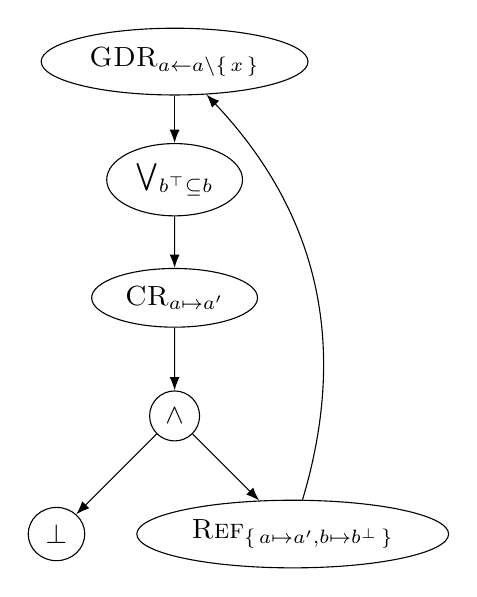
\begin{tikzpicture}[every node/.style={draw,ellipse},edge from
    parent/.style={draw,-Latex},sibling distance=3cm]
    \node (dr) {$\GDR_{a \gets a \setminus \{\, x \,\}}$}
    child {node {$\bigvee_{b^\top \subseteq b}$}
      child {node {$\CR_{a \mapsto a'}$}
        child {
          node[circle] {$\wedge$}
          child {node {$\bot$}}
          % _{(\emptyset, \{\, (X, Y) \,\}, \{\, X \mapsto b^\top, Y \mapsto b^\top \,\})}
          child {node (ref) {$\Reff_{\{\, a \mapsto a', b \mapsto b^{\bot} \,\}}$}}
        }}};
    \draw[-Latex, bend right] (ref) to (dr);
  \end{tikzpicture}
  \caption{A simplified version of an FCG constructed by \textsc{Crane} for the
    problem of counting partial injections from \cref{example:first}. Label
    $\bigvee_{b^\top \subseteq b}$ denotes set-disjunction, $\land$ denotes
    conjunction, and $\bot$ denotes a contradiction---see the work by
    \citet{DBLP:conf/ijcai/BroeckTMDR11} for the descriptions of these node
    types. Here we omit nodes whose only arithmetic effect is multiplication by
    one. Some of these nodes play an important role in the weighted version of
    the problem whereas others are remnants of the interaction between
    compilation rules and the way in which \textsc{ForcLift} handles existential
    quantifiers.}\label{fig:examplefcg}
\end{figure}

% From circuits to graphs.
A \emph{first-order deterministic decomposable negation normal form
  computational graph} (FCG) is a (weakly connected) directed graph with a
single source, node labels, and ordered outgoing edges.\footnote{Note that
  imposing an ordering on outgoing edges is just a limited version of edge
  labelling.} We denote an FCG as $G = (V, s, N^+, \tau)$, where $V$ is the set
of nodes, and $s \in V$ is the unique source. Function $N^+$ maps each node in
$V$ to a \emph{list} of its direct successors. Node labels consist of two parts:
the \emph{type} and the \emph{parameters}. To avoid clutter, we leave the
parameters implicit and let $\tau$ denote the node-labelling function that maps
each node in $V$ to its type. For each node $v \in V$, the length of list
$N^+(v)$ (i.e., the out-degree of $v$) is determined by its type $\tau(v)$. Most
of the types are as in previous work
\citep{DBLP:conf/nips/Broeck11,DBLP:conf/ijcai/BroeckTMDR11}. The type for
non-tree-like edges (denoted by $\Reff$), while used before, is extended to
contain the information necessary to support recursive calls. We also add three
new types:
\begin{itemize}
  \item a type for \emph{constraint removal} denoted by $\CR$,
  \item a type for \emph{generalised domain recursion} denoted by $\GDR$ (both
        with out-degree one),
  \item and $\star$---a placeholder type (with out-degree zero) for nodes that
        are going to be replaced.
\end{itemize}
When drawing an FCG, we order outgoing edges from left to right, write node
labels directly on the nodes, and omit irrelevant labels and/or parameters. See
\cref{fig:examplefcg} for an example FCG\@. Its source node has out-degree 1
(i.e., $|N^+(s)| = 1$), label $\GDR_{a \gets a \setminus \{\, x \,\}}$, and type
$\GDR$ (i.e., $\tau(s) = \GDR$).

%\paragraph*{Notation.}
Similarly to \citet{DBLP:conf/ijcai/BroeckTMDR11}, we write $T_p$ for an FCG
that has a node with label $T_p$ (i.e., type $T$ and parameter(s) $p$) and
$\star$'s as all of its direct successors. In particular, as an FCG, $\star$
denotes
$(\{\, s \,\}, s, \{\, s \mapsto \langle\rangle \,\}, \{\, s \mapsto \star \,\})$,
i.e., an FCG with just one node of type $\star$ and no edges. We write $T_p(v)$
for an FCG with one edge from a node labelled $T_{p}$ to some other node $v$
(and no other nodes or edges).

\begin{figure}[t]
  \centering
  \begin{subfigure}{0.49\linewidth}
    \centering
    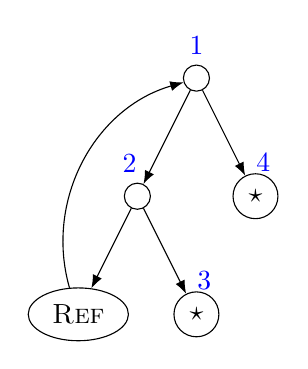
\begin{tikzpicture}[edge from parent/.style={draw,-Latex}]
      \node[draw,circle,label={[text=blue]1}] (top) {}
      child {
        node[draw,circle,label={[text=blue,xshift=-1mm]2}] {}
        child {node[draw,ellipse] (ref) {$\Reff$}}
        child {node[draw,circle,label={[text=blue,xshift=1mm,yshift=-1mm]3}] {$\star$}}
      }
      child {node[draw,circle,label={[text=blue,xshift=1mm,yshift=-1mm]4}] {$\star$}};
      \draw[-Latex] (ref) to [bend left=45] (top);
    \end{tikzpicture}
    \caption{An example FCG}\label{fig:smallexample1}
  \end{subfigure}
  \begin{subfigure}{0.49\linewidth}
    \centering
    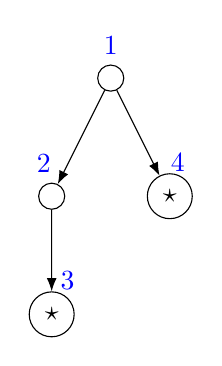
\begin{tikzpicture}[edge from parent/.style={draw,-Latex}]
      \node[draw,circle,label={[text=blue]1}] (top) {}
      child {
        node[draw,circle,label={[text=blue,xshift=-1mm]2}] {}
        child {node[draw,circle,label={[text=blue,xshift=2mm,yshift=-1mm]3}] {$\star$}}
      }
      child {node[draw,circle,label={[text=blue,xshift=1mm,yshift=-1mm]4}] {$\star$}};
    \end{tikzpicture}
    \caption{The underlying tree of
      \cref{fig:smallexample1}}\label{fig:smallexample2}
  \end{subfigure}
  \caption{An FCG and its underlying tree. The integers in blue denote the
    pre-order traversal of the underlying tree.}\label{fig:ordering}
\end{figure}

%\paragraph*{Connecting FCGs with formulas.}
Finally, we introduce a structure that represents a solution to a (W)FOMC
problem while it is still being built. A \emph{chip} is a pair $(G, L)$, where
$G$ is an FCG, and $L$ is a list of formulas, such that $|L|$ is equal to the
number of $\star$'s in $G$. The intuition behind this definition is that $L$
contains formulas that still need to be compiled. Once a formula is compiled, it
replaced one of the $\star$'s in $G$. We say that an FCG is \emph{complete}
(i.e., it represents a \emph{complete solution}) if it has no $\star$'s.
Similarly, a chip is complete if its FCG is complete (or, equivalently, the list
of formulas is empty). Let the \emph{underlying tree} of $G$ be the induced
subgraph of $G$ that omits all $\Reff$ nodes.\footnote{Subsequently presented
  algorithms ensure that the underlying tree is guaranteed to be a tree.} Then
we can define an implicit bijection between the formulas in $L$ and the
$\star$'s in $G$ according to the order in which elements of $L$ are listed and
the pre-order traversal of the underlying tree of $G$. For example, if $G$ is as
in \cref{fig:smallexample1} (with its underlying tree in
\cref{fig:smallexample2}), then $|L| = 2$. Moreover, the first element of $L$ is
associated with the $\star$ labelled 3, and the second with the one labelled 4.

\section{New Compilation Rules}\label{sec:rules}

A \emph{(compilation) rule} takes a formula and returns a set of chips. The
cardinality of this set is the number of different ways in which the rule can be
applied to the input formula. While \textsc{ForcLift}
\citep{DBLP:conf/ijcai/BroeckTMDR11} heuristically chooses one of them, in an
attempt to not miss a solution, \textsc{Crane} returns them all. In particular,
if a rule returns an empty set, then that rule is not applicable to the formula,
and the algorithm continues with the next rule.

\subsection{Generalised Domain Recursion}\label{sec:dr}
% 1. Note that the total number of such possibilities is not necessarily
% exponential: some combinations produce clearly unsatisfiable formulas that can
% be immediately discarded.
% 2. We can combine all of these possibilities into a single formula equivalent
% to the original one.
% 3. \begin{itemize}
%   \item the formula is shattered,
%   \item the formula has no independent subformulas,
%   \item and there exists a root binding class.
% \end{itemize}
% 4. During evaluation, $v$ is ignored, and the WMCs of $x$ and $r$ can be
% computed independently. Note that the WMC of $x$ is independent of the size of
% $D$---this further simplifies the matters.

% Main idea
The main idea behind domain recursion (both the original version by
\citet{DBLP:conf/nips/Broeck11} and the one presented here) is as follows. Let
$d \in \mathcal{D}$ be a domain. Assuming that $d \ne \emptyset$, pick some
$x \in d$. Then, for every variable $X$ associated with domain $d$ that occurs
in a literal, consider two possibilities: $X = x$ and $X \ne x$.

\begin{example}\label{example:dr}
  Let $\phi$ be a formula with a single clause
  \begin{multline*}
    (\{\, \neg p(X, Y), \neg p(X, Z) \,\}, \{\, (Y, Z) \,\}, \\
    \{\, X \mapsto a, Y \mapsto b, Z \mapsto b \,\}).
  \end{multline*}
  Then we can introduce constant $x \in a$ and rewrite $\phi$ as
  $\phi' = \{\, c_{1}, c_{2} \,\}$, where
  \begin{align*}
    c_{1} &= \begin{multlined}[t]
      (\{\, \neg p(x, Y), \neg p(x, Z) \,\}, \{\, (Y, Z) \,\}, \\
      \{\, Y \mapsto b, Z \mapsto b \,\}),
      \end{multlined}\\
    c_{2} &= \begin{multlined}[t]
      (\{\, \neg p(X, Y), \neg p(X, Z) \,\}, \{\, (X, x), (Y, Z) \,\}, \\
      \{\, X \mapsto a', Y \mapsto b, Z \mapsto b \,\}),
      \end{multlined}
  \end{align*}
  and $a' = a \setminus \{\, x \,\}$.
\end{example}

% Original domain recursion
\citet{DBLP:conf/nips/Broeck11} imposes stringent preconditions on the input
formula to ensure that the expanded version of the formula (as in
\cref{example:dr}) can be handled efficiently. The clauses in this expanded
formula are then partitioned into three parts based on whether the transformation
introduced constants or constraints or both. The aforementioned conditions
ensure that these parts can be treated independently.

\begin{algorithm}[t]
  \caption{The compilation rule for $\GDR$ nodes.}\label{alg:domainrecursion}
  \KwIn{formula $\phi$}
  \KwOut{set of chips $S$}
  $S \gets \emptyset$\;
  \ForEach{domain $d \in \mathcal{D}$ s.t.\ there is $c \in \phi$ and $v \in \Vars(L_c)$ s.t. $\delta_c(v) = d$\label{line:condition}}{
    $\phi' \gets \emptyset$\;
    $x \gets \text{a new constant in domain } d$\;
    \ForEach{clause $c = (L, C, \delta) \in \phi$\label{line:forclause}}{
      $V \gets \{\, v \in \Vars(L) \mid \delta(v) = d \,\}$\;
      \ForEach{subset $W \subseteq V$ s.t. $W^2 \cap C = \emptyset$ {\bf and} $W \cap \{\, v \in \Vars(C) \mid (v, y) \in C \text{ for some constant } y \,\} = \emptyset$\label{line:conditions}}{
        \tcc{$\delta'$ restricts $\delta$ to the new set of variables}
        $\phi' \gets \phi' \cup \{\, (L[x/W], C[x/W] \cup \{\, (v, x) \mid (v \in V \setminus W) \,\}, \delta') \,\}$\;\label{line:generation}
      }
    }
    $S \gets S \cup \{\, (\GDR_{d \gets d \setminus \{\, x \,\}}, \langle\phi'\rangle) \,\}$\;
  }
\end{algorithm}

% Description of GDR, in contrast to DR
In contrast, GDR has only one precondition: for GDR to be applicable on domain
$d \in \mathcal{D}$, there must be at least one variable with domain $d$ that is
featured in a literal (and not just in constraints). Without such variables, GDR
would have no effect on the formula. GDR is also simpler in that the expanded
formula is left as-is to be handled by other compilation rules. Typically, after
a few more rules are applied, a combination of $\CR$ and $\Reff$ nodes
introduces a loop back to the $\GDR$ node, thus completing the definition of a
recursive function. The GDR compilation rule is summarised as
\cref{alg:domainrecursion} and explained in more detail using the example below.

\begin{example}
  Let $\phi \coloneqq \{\, c_1, c_2 \,\}$ be the formula from
  \cref{example:first}. While GDR is possible on both domains, here we
  illustrate how it works on $a$. Having chosen a domain, the algorithm iterates
  over the clauses of $\phi$. Suppose \cref{line:forclause} picks $c = c_1$ as
  the first clause. Then, set $V$ is constructed to contain all variables with
  domain $d = a$ that occur in the literals of clause $c$. In this case,
  $V = \{\, X \,\}$.

  \Cref{line:conditions} iterates over all subsets $W \subseteq V$ of variables
  that can be replaced by a constant without resulting in formulas that are
  evidently unsatisfiable. We impose two restrictions on $W$. First,
  $W^2 \cap C = \emptyset$ ensures that there are no pairs of variables in $W$
  that are constrained to be distinct, since that would result in a $x \ne x$
  constraint after substitution. Similarly, we want to avoid variables in $W$
  that have inequality constraints with constants: after substitution, such
  constraints would transform into inequality constraints between two constants.
  In this case, both subsets of $V$ satisfy these conditions, and
  \cref{line:generation} generates two clauses for the output formula:
  \begin{multline*}
    (\{\, \neg p(X, Y), \neg p(X, Z) \,\}, \{\, (Y, Z), (X, x) \,\}, \\
    \{\, X \mapsto a, Y \mapsto b, Z \mapsto b \,\}),
  \end{multline*}
  from $W = \emptyset$ and
  \[
    (\{\, \neg p(x, Y), \neg p(x, Z) \,\}, \{\, (Y, Z) \,\}, \{\, Y \mapsto b, Z \mapsto b \,\})
  \]
  from $W = V$.

  When \cref{line:forclause} picks $c = c_2$, then $V = \{\, X, Z \,\}$. The
  subset $W = V$ fails to satisfy the conditions on \cref{line:conditions}
  because of the $X \ne Z$ constraint. The other three subsets of $V$ all
  generate clauses for $\phi'$. Indeed, $W = \emptyset$ generates
  \begin{multline*}
    (\{\, \neg p(X, Y), \neg p(Z, Y) \,\}, \{\, (X, Z), (X, x), (Z, x) \,\}, \\
    \{\, X \mapsto a, Y \mapsto b, Z \mapsto a \,\}),
  \end{multline*}
  $W = \{\, X \,\}$ generates
  \[
    (\{\, \neg p(x, Y), \neg p(Z, Y) \,\}, \{\, (Z, x) \,\}, \{\, Y \mapsto b, Z \mapsto a \,\}),
  \]
  and $W = \{\, Z \,\}$ generates
  \[
    (\{\, \neg p(X, Y), \neg p(x, Y) \,\}, \{\, (X, x) \,\}, \{\, X \mapsto a, Y \mapsto b \,\}).
  \]
\end{example}

\subsection{Constraint Removal}\label{sec:cr}

\begin{algorithm}[t]
  \caption{The compilation rule for $\CR$ nodes.}\label{alg:constraintremoval}
  \KwIn{formula $\phi$, set of domains $\mathcal{D}$}
  \KwOut{set of chips $S$}
  $S \gets \emptyset$\;
  \ForEach{domain $d \in \mathcal{D}$ and element $x \in d$ s.t. $x$ does not occur in any literal of any clause of $\phi$ {\bf and} for each clause $c = (L, C, \delta_c) \in \phi$ and variable $v \in \Vars(c)$, either $\delta_c(v) \ne d$ or $(v, x) \in C$\label{line:crconditions}}{
    add a new domain $d'$ to $\mathcal{D}$\;
    $\phi' \gets \emptyset$\;
    \ForEach{clause $(L, C, \delta) \in \phi$}{
      $C' \gets \{\, (a, b) \in C \mid b \ne x \,\}$\;\label{line:constraintremoval}
      \nosemic$\delta' \gets v \mapsto \begin{cases} d' & \text{if} \delta(v) = d\\ \delta(v) & \text{otherwise;} \end{cases}$\;\label{line:newdelta}
      $\phi' \gets \phi' \cup \{\, (L, C', \delta') \,\}$\;
    }
    $S \gets S \cup \{\, (\CR_{d \mapsto d'}, \langle\phi'\rangle) \,\}$\;
  }
\end{algorithm}

Recall that GDR on a domain $d$ creates constraints of the form $X_i \ne x$ for
some constant $x \in d$ and family of variables $X_i \in d$. Once certain
conditions are satisfied, \cref{alg:constraintremoval} can eliminate these
constraints and replace $d$ with a new domain $d'$, which can be interpreted as
$d \setminus \{\, x \,\}$. These conditions (on \cref{line:crconditions} of the
algorithm) are that a constraint of the form $X \ne e$ exists for all variables
$X \in d$ across all clauses, and such constraints are the only place where $e$
occurs. The algorithm then proceeds to construct the new formula by removing
constraints (on \cref{line:constraintremoval}) and constructing a new domain map
$\delta'$ that replaces $d$ with $d'$ (on \cref{line:newdelta}).

\begin{example}
  Let $\phi = \{\, c_1, c_2, c_3 \,\}$ be a formula with clauses
  \begin{align*}
    c_1 &= (\emptyset, \{\, (Y, X) \,\}, \{\, X \mapsto b^\top, Y \mapsto b^\top \,\}), \\
    c_2 &=
          \begin{multlined}[t]
            (\{\, \neg p(X, Y), \neg p(X, Z) \,\}, \{\, (X, x), (Y, Z) \,\}, \\
            \{\, X \mapsto a, Y \mapsto b^\bot, Z \mapsto b^\bot \,\}),
          \end{multlined}\\
    c_3 &=
          \begin{multlined}[t]
            (\{\, \neg p(X, Y), \neg p(Z, Y) \,\}, \{\, (X, x), (Z, X), (Z, x) \,\}, \\
            \{\, X \mapsto a, Y \mapsto b^\bot, Z \mapsto a \,\}).
          \end{multlined}
  \end{align*}
  Domain $a$ and with its element $x \in a$ satisfy the preconditions for
  constraint removal. The rule introduces a new domain $a'$ and transforms
  $\phi$ to $\phi' = (c_1', c_2', c_3')$, where
  \begin{align*}
    c_1' &= c_1, \\
    c_2' &=
           \begin{multlined}[t]
             (\{\, \neg p(X, Y), \neg p(X, Z) \,\}, \{\, (Y, Z) \,\}, \\
             \{\, X \mapsto a', Y \mapsto b^\bot, Z \mapsto b^\bot \,\}),
           \end{multlined} \\
    c_3' &=
           \begin{multlined}[t]
             (\{\, \neg p(X, Y), \neg p(Z, Y) \,\}, \{\, (Z, X) \,\}, \\
             \{\, X \mapsto a', Y \mapsto b^\bot, Z \mapsto a' \,\}).
           \end{multlined}
  \end{align*}
\end{example}

\subsection{Identifying Opportunities for Recursion}\label{sec:ref}

TODO: write a short informal summary. Add the full info as an appendix and
reference it.

\section{How to Interpret an FCG}\label{sec:interpret}

When \textsc{ForcLift} \citep{DBLP:conf/ijcai/BroeckTMDR11} compiles a WFOMC
instance into a circuit, each gate type encodes an arithmetic operation on its
inputs and parameters. These operations are then immediately performed while
traversing the circuit and using domain sizes and weights as the initial inputs.
With \textsc{Crane}, the interpretation of an FCG is a collection of functions.
Each function has (some) domain sizes as parameters and may contain recursive
calls to other functions, including itself. While there may be any number of
subsidiary functions, there is always one main function that can be called with
the sizes of the domains of the input formula as arguments. Henceforth, this
function is always called $f$, and it is defined by the source node.

The interpretation of a node is decided by its type. Here we describe the
interpretations of new (or significantly changed) types and refer the reader to
previous work \citep{DBLP:conf/ijcai/BroeckTMDR11} for information on other
types. Both $\CR$ and $\GDR$ nodes do not contribute anything to the definitions
of functions---the interpretation of such a node is simply the interpretation of
its only direct successor. Obviously, $\star$ nodes also have no interpretation,
although for a different reason: incomplete FCGs are not meant to be
interpreted. The interpretation of a $\Reff$ node is a function call. The direct
successor of the $\Reff$ node (say, $v$) then must introduce a function. The
parameters of this function are the sizes of all domains used by nodes reachable
from $v$.

\begin{example}\label{example:interpretation}
  Let us use the FCG from \cref{fig:examplefcg} as an example. The input formula
  (i.e., the formula in \cref{example:first}) has two domains: $a$ and $b$.
  Thus, the interpretation of the FCG is a function
  $f\colon \mathbb{N}_{0} \times \mathbb{N}_{0} \to \mathbb{R}_{\ge 0}$. Let
  $m \coloneqq |a|$, and $n \coloneqq |b|$. The node labelled
  $\bigvee_{b^{\top} \subseteq b}$ tells us that
  $f(m, n) = \sum_{l = 0}^{n} \binom{n}{l} \square$, where $\square$ is the
  interpretation of the remaining subgraph, and $l$ iterates over all possible
  sizes of $b^{\top}$. It also creates two subdomains
  $b^{\top}, b^{\bot} \subseteq b$ that partition $b$, i.e., as the size of
  $b^{\top}$ increases, the size of $b^{\bot}$ correspondingly decreases. Nodes
  labelled $\land$ correspond to multiplication. Therefore,
  $f(m, n) = \sum_{l = 0}^{n} \binom{n}{l} \diamondsuit \times \heartsuit$,
  where $\diamondsuit$ is the interpretation of the contradiction (i.e., $\bot$)
  node, and $\heartsuit$ is the interpretation of the $\Reff$ node.

  A contradiction node with clause $c$ as a parameter is interpreted as one if
  the clause has groundings and zero otherwise. In this case, the parameter is
  $c = (\emptyset, \{\, (X, Y) \,\}, \{\, X \mapsto b^\top, Y \mapsto b^\top \,\})$
  (not shown in \cref{fig:examplefcg}), which can be read as
  $\forall X, Y \in b^{\top}\text{. }X \ne Y \implies \bot$, i.e.,
  $\forall X, Y \in b^{\top}\text{, }X = Y$. This latter sentence is true if and
  only if $|b^{\top}| < 2$. Therefore, we can use the Iverson bracket notation
  to write
  \[
    \diamondsuit = [l < 2] \coloneqq
    \begin{cases}
      1 & \text{if } l < 2 \\
      0 & \text{otherwise.}
    \end{cases}
  \]

  It remains to interpret the $\Reff$ node. Parameter
  $\{\, a \mapsto a', b \mapsto b^\bot \,\}$ tells us that the interpretation of
  the $\Reff$ node should be the same as that of the source node, but with
  domains $a$ and $b$ replaced with $a'$ and $b^{\bot}$, respectively. Domain
  $a'$ was created by a constraint removal rule applied on $a$, so
  $|a'| = m - 1$. Now $b^{\bot} = b \setminus b^{\top}$, and $|b^{\top}| = l$,
  so $|b^{\bot}| = n - l$. Thus, the interpretation of the $\Reff$ node is a
  recursive call to $f(m - 1, n - l)$. Therefore,
  \begin{align}
    f(m, n) &= \sum_{l = 0}^{n} \binom{n}{l} [l < 2] f(m-1, n-l)\nonumber \\
            &= f(m-1, n) + n f(m-1, n-1).\label{eq:solution}
  \end{align}
  In order to use this recursive function to compute the model count of the
  input formula for any domain sizes, one just needs to find the base cases
  $f(0, n)$ and $f(m, 0)$ for all $m, n \in \mathbb{N}_{0}$.
\end{example}

\section{Empirical Results}\label{sec:results} % Newly Domain-Liftable Formulas

\begin{table*}[t]
  \centering
  \begin{tabular}{cccccc}
    \toprule
    \multicolumn{3}{c}{Function Class} & \multicolumn{3}{c}{Asymptotic Complexity of Counting} \\
    Partial & Endo- & Class & Best Known & With \textsc{ForcLift} & With \textsc{Crane} \\
    \midrule
    \rowcolor{gray!10}\cmark/\xmark & \cmark/\xmark & Functions & $\log m$ & $m$ & $m$ \\
    \xmark & \xmark & \multirow{4}{*}{Surjections} & $n \log m$ & $m^{3}+n^{3}$ & $m^{3}+n^{3}$ \\
    \xmark & \cmark & & $m \log m$ & $m^{3}$ & $m^{3}$ \\
    \cmark & \xmark & & \multicolumn{3}{c}{Same as injections from $b$ to $a$} \\
    \cmark & \cmark & & \multicolumn{3}{c}{Same as endo-injections} \\
    \rowcolor{gray!10}\xmark & \xmark & & $m$ & --- & $mn$ \\
    \rowcolor{gray!10}\xmark & \cmark & & $m$ & --- & $m^3$ \\
    \rowcolor{gray!10}\cmark & \xmark & & $\min\{\, m, n \,\}^2$ & --- & $mn$ \\
    \rowcolor{gray!10}\cmark & \cmark & \multirow{-4}{*}{Injections} & $m^2$ & --- & --- \\
    \xmark & \xmark & \multirow{3}{*}{Bijections} & $m$ & --- & $m$ \\
    \xmark & \cmark & & \multicolumn{3}{c}{\multirow{2}{*}{Same as (partial) (endo-)injections}} \\
    \cmark & \cmark/\xmark & & \multicolumn{3}{c}{} \\
    \bottomrule
  \end{tabular}
  \caption{The worst-case complexity of counting various types of functions.
    Here, $m$ is the size of domain $a$, and $n$ is the size of domain $b$. All
    asymptotic complexities are in $\Theta(\cdot)$. A dash means that no
    complete solution was found.}\label{tbl:results}
\end{table*}

In this section, we compare \textsc{Crane} and \textsc{ForcLift}
\citep{DBLP:conf/ijcai/BroeckTMDR11} on their ability to count various kinds of
functions. (Other WFOMC algorithms such as \textsc{L2C}
\citep{DBLP:conf/kr/KazemiP16} and probabilistic theorem proving
\citep{DBLP:journals/cacm/GogateD16} are unable to solve any of the instances
that \textsc{ForcLift} fails on.) We begin by describing how such functions can
be expressed in FOL\@. \textsc{ForcLift} then translates these sentences in FOL
to formulas as defined in \cref{def:formula}.

% Describe what kind of instances we're investigating
Let $p \in a \times b$ be a predicate. To restrict all relations representable
by $p$ to just functions from $a$ to $b$, in FOL one might write
\[
  \forall X \in a\text{. }\forall Y, Z \in b\text{. }p(X, Y) \land p(X, Z) \implies Y = Z
\]
and
\begin{equation}\label{eq:def2}
  \forall X \in a\text{. }\exists Y \in b\text{. }p(X, Y).
\end{equation}
The former sentence says that one element of $a$ can map to at \emph{most} one
element of $b$, and the latter sentence says that each element of $a$ must map
to at \emph{least} one element of $b$. One can then add
\[
  \forall W, X \in a\text{. }\forall Y \in b\text{. }p(W, Y) \land p(X, Y) \implies W = X
\]
to restrict $p$ to injections or
\[
  \forall Y \in b\text{. }\exists X \in a\text{. }p(X, Y)
\]
to ensure surjectivity or remove \cref{eq:def2} to consider partial functions.
Lastly, one can replace all occurrences of $b$ with $a$ to model endofunctions
(i.e., functions with the same domain and codomain) instead.

% the process: both for running algorithms and for determining complexities
In our experiments, we consider all sixteen combinations of these properties,
i.e., injectivity, surjectivity, partiality, and endo-. \textsc{ForcLift} is
always run until it terminates. \textsc{Crane} is run until either five
solutions are found or the search tree reaches height 6.\footnote{The search
  tree has a high branching factor, so exploring all nodes at depth 5 takes at
  most a few seconds whereas doing the same for depth 6 can be computationally
  infeasible in some cases.} If successful, \textsc{ForcLift} generates a
circuit, and \textsc{Crane} generates one or more (complete) FCGs. In both
cases, we manually convert the resulting graphs into definitions of functions as
described in \cref{sec:interpret}. We then assess the complexity of each
solution and pick the best if \textsc{Crane} returns several solutions of
varying complexities. When assessing the complexity of each such definition, we
make two assumptions. First, we can compute the binomial coefficient
$\binom{n}{k}$ in $\Theta(nk)$ time. Second, techniques such as dynamic
programming and memoization are used to avoid recomputing the same binomial
coefficient or function call multiple times.

The experimental results are summarised in \cref{tbl:results}. The best-known
asymptotic complexity for computing total surjections is by \citet{30049}. All
other best-known complexity results are inferred from the formulas and programs
on the on-line encyclopedia of integer sequences \citep{oeis}. On instances that
could already be solved by \textsc{ForcLift}, the two algorithms perform equally
well. However, \textsc{Crane} is also able to solve all but one instances that
\textsc{ForcLift} fails on in at most cubic time.

Let us examine the case of counting partial (non-endomorphic) injections more
closely. The FCG in \cref{fig:examplefcg,example:interpretation} counts partial
injections and is responsible for the $mn$ entry in the table. For a complete
solution, \cref{eq:solution} must be combined with the base case $f(0, n) = 1$
for all $n \in \mathbb{N}_{0}$. In other words, the base case says that the
empty partial map is the only partial injection with an empty domain, regardless
of the codomain. Finally, note that $f(m, n)$ can be evaluated in $\Theta(mn)$
time by a dynamic programming algorithm that computes $f(i, j)$ for all
$i = 0, \dots, m$ and $j = 0, \dots, n$.

  % \item The complexities assume that arithmetic operations on number such as
  %       addition and multiplication take constant time.
  % \item In some cases (e.g., when counting injections from... to...), we might
  %       immediately recognize that the answer must be zero. Whether such cases
  %       can be handled efficiently or not by our approach depends on the
  %       definitions of functions and the order of evaluation. (We still get the
  %       right answer, though.)
  % \item All complexity results are for the worst case. In particular, optimal
  %       best-case complexity is usually $\Theta(1)$ (see above for why).

% Other results
% \begin{itemize}
%   \item 1d bijections and 1d injections (note that it's the same problem). Depth
%         3 solution:
%         \begin{align*}
%           f(n) &= \sum_{m=0}^n \binom{n}{m} (-1)^{n-m}g(n, m) \\
%           g(n, m) &= \sum_{l=0}^n \binom{n}{l}[l < 2]g(n-l, m-1) \\
%                &= g(n, m - 1) + ng(n - 1, m - 1),
%         \end{align*}
%         which works with base case $g(n, 0) = 1$.
%   \item 1d partial injections. 2 solutions at depth 6, but they're too
%         complicated to check by hand. A contradiction with $X \ne x$ constraints
%         makes things complicated.
%   \item 2d bijections. Depth 3:
%         \begin{align*}
%           f(m, n) &= \sum_{l=0}^m \binom{m}{l} [l < 2] (1 - [l < 1])f(m-l, n-1) \\
%                   &= mf(m-1, n-1),
%         \end{align*}
%         which works with base cases $f(0, 0) = 1$, $f(0, n) = 0$, $f(m, 0) = 0$.
%   \item 2d partial injections, depth 2. Exactly the same circuit as for injections but with base case $f(m, 0) = 1$.
% \end{itemize}

\section{Conclusion and Future Work}

% A summary of what's been done/achieved and how

In this paper, we showed how a state-of-the-art (W)FOMC algorithm can be
empowered by generalising domain recursion and adding support for cycles in the
graph that encodes a solution. To construct such graphs, \textsc{Crane}
supplements \textsc{ForcLift} \citep{DBLP:conf/ijcai/BroeckTMDR11} with three
new compilation rules and a hybrid search algorithm. In \cref{sec:results}, we
saw examples of instances that become liftable not just in theory
\citep{DBLP:journals/jair/Kuzelka21} but with an implemented algorithm as well.
However, our experiments cover only a small set of instances since some parts of
\textsc{Crane} are yet to be fully automated. Specifically, our experiments
focus on various function-counting problems---it remains to be seen what other
types of instances become liftable as a result.

% An idea pivotal to our work is the generalisation of circuits to graphs. Despite
% the wide variety of circuits that are used in artificial intelligence
% \citep{DBLP:series/faia/Darwiche21}, this is the first time that the addition of
% cycles is shown to make a class of circuits more powerful. An important strand
% for future work is in developing an algorithm that learns FCGs from data
% similarly to the way \textsc{ForcLift} has been utilised in learning Markov
% logic networks \citep{DBLP:conf/aaai/BroeckMD13,DBLP:journals/ml/HaarenBMD16}.
% One could also consider whether some of the many recent applications of circuits
% are suitable for FCGs as well. These applications include the verification and
% explainability of neural networks \citep{DBLP:conf/pods/Darwiche20}, causal
% inference \citep{https://doi.org/10.48550/arxiv.2202.02891}, computing the
% expectations of kernel functions \citep{DBLP:conf/uai/LiZVB21}, and variational
% inference in discrete graphical models \citep{DBLP:conf/nips/ShihE20}.

However, the most important direction for future work is in fully automating
this new way of computing the (W)FOMC of a formula. First, we need an algorithm
that transforms FCGs into definitions of functions. Formalising this process
would also allow us to prove the correctness of the new compilation rules in
constructing FCGs that indeed compute the right WMC\@. Second, these definitions
must be simplified before they can be used, perhaps by a computer algebra
system. Third, most importantly, we need a way to find the base cases for the
recursive definitions provided by \textsc{Crane}. What makes this problem
non-trivial is that the number of base cases is not constant for functions of
arity greater than one (i.e., formulas that mention more than one domain). On
the other hand, assuming that a domain is empty can greatly simplify a problem.
Fourth, since the first solution found by \textsc{Crane} is not always optimal
in terms of its complexity, an automated way to determine the asymptotic
complexity of a solution would be helpful as well. Achieving these goals would
make \textsc{Crane} capable of automatically constructing efficient ways to
compute a function (e.g., a sequence) of interest. In addition to the potential
impact to areas of artificial intelligence (AI) such as statistical relational
AI \citep{DBLP:series/synthesis/2016Raedt}, \textsc{Crane} could be beneficial
to research in combinatorics as well \citep{DBLP:conf/ilp/BarvinekB0ZK21}.

\bibliography{paper}
\end{document}
